\chapter{基于多主题矩阵分解的评分预测}
\label{chapter-bpmtmf}
本章重点介绍针对显式评分数据进行\textit{评分预测}的研究内容。首先,章节~\ref{sec-bpmtmf-intro}描述本章的研究内容和大概的解决思路。接着,章节~\ref{sec-bpmtmf-model}具体介绍本章提出的评分预测模型及其优化算法,并描述了模型与现有的局部矩阵分解模型之间的联系。随后在章节~\ref{sec-bpmtmf-experiments}中分析基于两个电影评分数据集上的实验结果。最后总结本章工作研究内容。

\section{引言}
\label{sec-bpmtmf-intro}


上一章介绍了个性化推荐系统的一个典型任务\textit{商品推荐},即根据用户的历史行为信息推荐用户感兴趣的商品。本章节介绍个性化推荐系统的另一个典型任务\textit{评分预测},是基于用户历史的显式评分数据预测用户对给定商品的评分,用以表达用户对商品的满意程度。第~\ref{chapter:relatedwork}章中介绍了大量的\textit{评分预测}模型,其中章节~\ref{sec-related-pmf}详细介绍了一个针对\textit{评分预测}的经典模型,概率矩阵分解模型(PMF)~\cite{salakhutdinov2007probabilistic}。该模型在许多真实竞赛中拥有良好的表现,例如Netflix百万美元竞赛得主的模型中的一个主要模型就是矩阵分解。PMF利用零均值球面高斯分布作为隐藏特征的先验分布,使用高斯分布对评分信息建模,将用户和商品属性投射到低秩空间中,然后使用用户和商品隐藏特征向量的点积还原评分矩阵的缺失值。近期,针对\textit{评分预测}任务的局部矩阵分解模型~\cite{lee2013local}已被验证比传统的矩阵分解模型更加有效。它的主要思想是将原始评分矩阵分成几个较小的子矩阵,然后利用局部结构来获得更好的低秩近似。然后在每个子矩阵中,应用标准矩阵分解技术来为用户和商品生成子矩阵特定的隐藏特征向量。通常,使用聚类技术获得这些子矩阵。通过组合多个子矩阵$\mathbf{\mathbf{R}^1,\mathbf{R}^2,..., \mathbf{R}^H}$以及对应的权重$\{\mathbf{V}^1,\mathbf{V}^2,...,\mathbf{V}^H\}$重新构成原始矩阵$\mathbf{R}$:

\begin{equation}
\label{eq-bpmtmf-localmf}
\hat{\mathbf{R}}_{um}= \frac{1}{\mathbf{Z}_{um}}\sum_{h=1}^H \mathbf{V}_{um}^{h}\mathbf{R}_{um}^{h}
\end{equation}
其中$\mathbf{Z}_{um}=\sum_{h=1}^H\mathbf{V}_{um}^h$是归一化因子,$\mathbf{V}_{um}^h$代表了项$\mathbf{R}_{um}^h$在子矩阵$\mathbf{R}^h$中的权重。在第\ref{chapter-lwmf}章已经说明这类矩阵集成的方法主要有两个关键问题:1)如何产生子矩阵和(2)如何设置子矩阵的集合权重。当前已经有一些工作去解决这两点,例如使用随机抽样~\cite{MJT11},使用锚点扩展最近邻数据点~\cite{lee2013local,lee2014local},或者基于联合硬聚类分割的方法~\cite{chen2015wemarec}。

虽然这些研究在某种程度上比传统矩阵分解模型有所改进,但缺乏一种更可信的方法来表示局部矩阵分解。通过回顾以前的研究~\cite{MJT11,lee2013local,lee2014local,chen2015wemarec},有两个重要的发现:(1)每个子矩阵可以被认为是用户和商品的局部聚类; (2)用户或商品在不同子矩阵中具有多个隐藏特征表示。受这两个观察的启发,本章提出一种新颖的贝叶斯概率多主题矩阵因子分解模型(Bayesian Probabilistic Multi- Topic Matrix Factorization ,简称BPMTMF)来进行\textit{评分预测}。本章的模型包括两个部分,即对用户访问商品行为建模和对评分建模。对于第一部分,本章将用户访问过的商品视为一个文档,并且利用主题模型中主题来``聚类''商品,每个主题是关于商品的多项式分布。随后,用户具有在主题集合上的多项式分布(即主题分布)。基于这样的主题,本章进一步为用户和商品设置主题特定的隐藏特征向量。本章工作将以一个完整的贝叶斯方法整合上述两个部分。本章提出模型的最终评分预测是由各个主题特定的隐藏特征向量生成的评分组合而成。本章节模型使用贝叶斯概率的方法描述了公式~\ref{eq-bpmtmf-localmf}的思想,即每个主题被认为是一个聚类。使用多主题隐藏特征表示,本章模型能更好地反映用户和商品在\textit{评分预测}中的复杂特性。使用主题模型的另一个重要优点是BPMTMF具有更好的模型可解释性。由于主题模型能够有效地发现共现的主题语义~\cite{blei2003latent},BPMTMF中产生的相同主题的商品也是高度相关的。使用此类方法,一个主题得到的商品也比以前的研究~\cite{MJT11,lee2013local,lee2014local,chen2015wemarec}中获得的更加一致。将主题作为上下文信息,本章工作可以分析用户的评分喜好在不同的主题中是如何变化的。

值得注意的是,在现有研究工作中研究人员已经做了一些将主题模型与矩阵分解模型结合的尝试,包括CTM~\cite{wang2011collaborative},HFT~\cite{mcauley2013hidden}和ETF~\cite{zhang2014explicit}。然而,这些方法主要是将评分结合到文本信息的主题模型中,并且期望结合两种模型的优点。通常,这类模型使用单个全局的矩阵分解模型建模评分数据,因此其不适合于局部矩阵分解模型。因此本章工作是针对显式评分数据第一次提出了一种局部矩阵分解的贝叶斯模型,它将主题模型与概率矩阵分解模型结合起来。通过使用主题作为聚类依据使得模型有更好的可解释性。在大型真实世界数据集的实验表明了所提出的模型与多个竞争性基线模型相比具有更高的评分预测有效性。

% \section{相关工作}
% 在本节中,我们将回顾相关工作。

% 矩阵因式分解。 MF [Paterek,2007; Mnih和Salakhutdinov,2007; Koren等人,2009]是一种重要的基于模型的协同过滤方法。 MF通过将用户和项目投影到潜在的低维空间中来构造低秩近似。 此外,已经通过使用高斯分布来建模具有零均值球面高斯先验的观察到的评级的概率矩阵因子分解(PMF)。 实质上,PMF可以被认为是规则化奇异值分解的概率实现。 此外,Salakhutdinov和Mnih [Salakhutdinov和Mnih,2008]提出了一个完整的贝叶斯公式PMF。 由于MF,双向MF和SVD ++的扩展已经在[Koren等人,2009]中提出。 偏置MF包括用户偏好和项目偏差,而SVD ++使用隐式反馈来改善用户偏好建模。

% 最近,几个关于使用子矩阵集合进行更好低阶近似的研究,包括DFC [Mackey et al。,2011],LLORMA [Lee et al。,2013; 2014],ACCAMS [Beutel等,2015]和WEMAREC [Chen等,2015]。这些方法将原始矩阵分割成若干较小的子矩阵,并且将单独的局部MF应用于每个子矩阵。使用多个局部MF的集合获得最终预测。通常,使用启发式适配的基于聚类的技术用于子矩阵生成。我们简要回顾这些研究。 Mackey et al。 [Mackey et al。,2011]引入了一个除法因子组合(DFC)框架,其中矩阵分解的昂贵任务被随机分为较小的子问题。 LLORMA [Lee et al。,2013; 2014]使用非参数核平滑方法搜索最近邻; WEMAREC [Chen et al。,2015]采用Bregman共聚类[Dhillon et al。,2003]技术分割原始矩阵; ACCAMS采用加法共聚类方法[Shan and Baner-jee,2008]来推导子矩阵并使用高斯分布来预测等级。我们的工作是建立在上述研究基础上的,然而,我们建议使用概率主题模型来创建“软”聚类,通过将主题模型与概率MF相结合,进一步开发一个完整的贝叶斯模型。

% 与主题模型的矩阵因式分解。在文献中,研究人员已经做了几项将主题模型与MF结合的尝试,包括CTM [Wang and Blei,2011],HFT [McAuley和Leskovec,2013]和ETF [Zhang et al。,2014]。然而,这些方法主要旨在将评级结合到主题模型中,并且集中于组合来自两种模型的优点。通常,使用单个MF分量,其不适合于本地MF。


% \subsection{概率潜在语义分析}\label{sec:plsa}
% 概率潜在语义分析(PLSA)\cite{Hofmann1999}是一种主题模型(topic  model)。主题模型是对文字隐含主题进行建模的方法。它克服了传统信息检索中文档相似度计算方法的缺点,并且能够在海量互联网数据中自动寻找出文字间的语义主题。和基于奇异值分解的隐语义分析不同,PLSA是一个生成模型,因此基于统计学的推论方法,最大似然方法\cite{Moon1996} 均可以用来学习模型参数。
% \begin{figure*}[htbp]
% 	\centering
% 	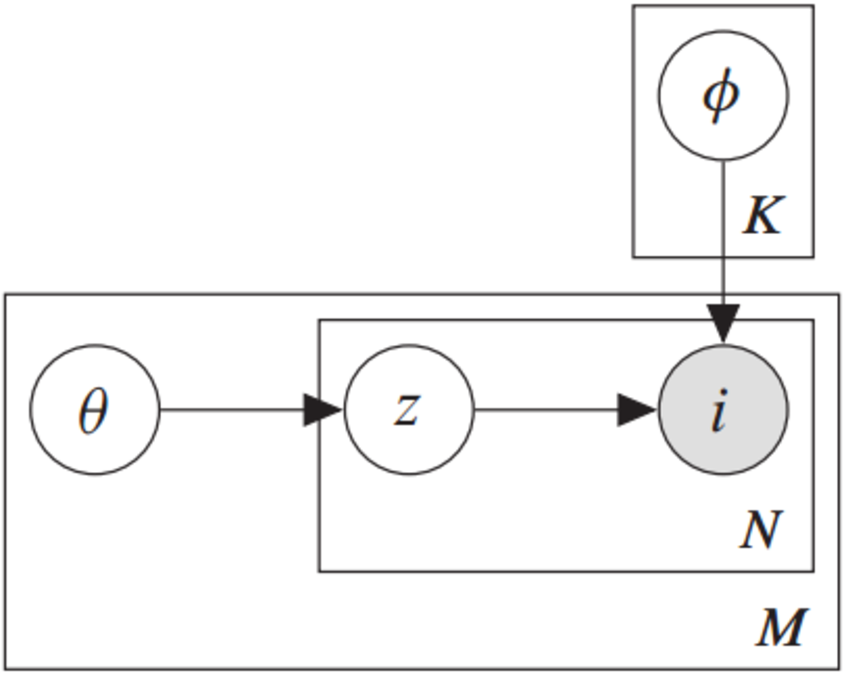
\includegraphics[width=0.4\textwidth]{Fig/bpmtmf/plsa}	
% 	\caption{概率隐藏语义分析}
% 	\label{fig-bpmtmf-plsa}
% \end{figure*}

% 图\ref{plsa}是PLSA的图模型表示。M表示用户个数,N表示POI 的个数。$\theta$是每个用户的主题的先验分布。给定一个用户u,多项式分布$\theta_u$表示该用户各个主题的分布。多项式分布$\phi_k$ 表示主题k中POI的分布。生成过程如下:
% \begin{itemize}
% 	\item 对每个用户u:
% 	\begin{itemize}
% 		\item 对$n_u$个POI采样
% 		\item 对每个$s \in {i,...,n_u}$
% 		\begin{itemize}
% 			\item z~DISC($\Theta_u$)
% 			\item 选择一个POI p~DISC($\Phi_z$)
% 		\end{itemize}
% 	\end{itemize}
% \end{itemize}

% 概率公式如公式\ref{equ:pgm2},\ref{equ:pgm3}:
% \begin{equation}
% P(d_i,w_j)=P(d_i)P(w_j|d_i)
% \label{equ:pgm2}
% \end{equation}
% \begin{equation}
% P(w_j|d_i)=\sum_{k=1}^{K}P(w_j|z_k)P(z_k|d_i)
% \label{equ:pgm3}
% \end{equation}

% PLSA的EM求解如下:

% E步如公式\ref{equ:pgm4}:
% \begin{equation}
% \gamma(z_ijk)=p(z_k|d_i,w_j)=\frac{p(d_i)p(z_k|d_i)p(w_j|z_k)}{\sum_{k=1}^{K}p(z_k|d_i)p(w_j|z_k)}=\frac{p(z_k|d_i)p(w_j|z_k)}{\sum_{k=1}^{K}p(z_k|d_i)p(w_j|z_k)}
% \label{equ:pgm4}
% \end{equation}

% M步如公式\ref{equ:pgm5},\ref{equ:pgm6}:
% \begin{equation}
% p(w_j|z_k)=\frac{\sum_{i=1}^{N}n(d_i,w_j)P(z_k|d_i,w_j)}{\sum_{m=1}^{M}\sum_{i=1}^{N}n(d_i,w_m)P(z_k|d_i,w_m)}
% \label{equ:pgm5}
% \end{equation}
% \begin{equation}
% p(z_k|d_i)=\frac{\sum_{j=1}^{M}n(d_i,w_j)P(z_k|d_i,w_j)}{n(d_i)}
% \label{equ:pgm6}
% \end{equation}

% 卡尔加里大学的一篇论文中\cite{Zhou2012}将基于内存的两种推荐方法(基于用户的和基于内存的)以及PLSA 进行对比,实验评估精度和召回两个指标,实验结果表明PLSA一直表现好于两周基于内存的推荐方法。

% 与基于内存的推荐算法相比,PLSA不依赖于相似度计算,用一种概率的方式解释了用户对POI 的签到行为。
% \subsection{隐含狄利克雷分布}
% 上一节提到的PLSA方法依赖于最大似然估计且没有对似然$\theta$做假设,所有的θ是等概率的,因此最优的参数集是由观察到的数据确定的。PLSA主要的缺点是参数的数量和数据集的大小成比例,并且没有合适的方法处理不可见的数据点。因此,贝叶斯学派提出隐含狄利克雷分布(Latent Dirichlet Allocation,LDA)\cite{Blei2003}。

% PLSA中Φ和θ是模型的参数,对应多项式分布,根据:

% Dirichlet先验+多项式分布的数据→后验分布为Dirichlet分布

% 所以在LDA中,为$\phi$和$\theta$增加Dirichlet先验分布。
% \begin{figure*}[htbp]
% 	\centering
% 	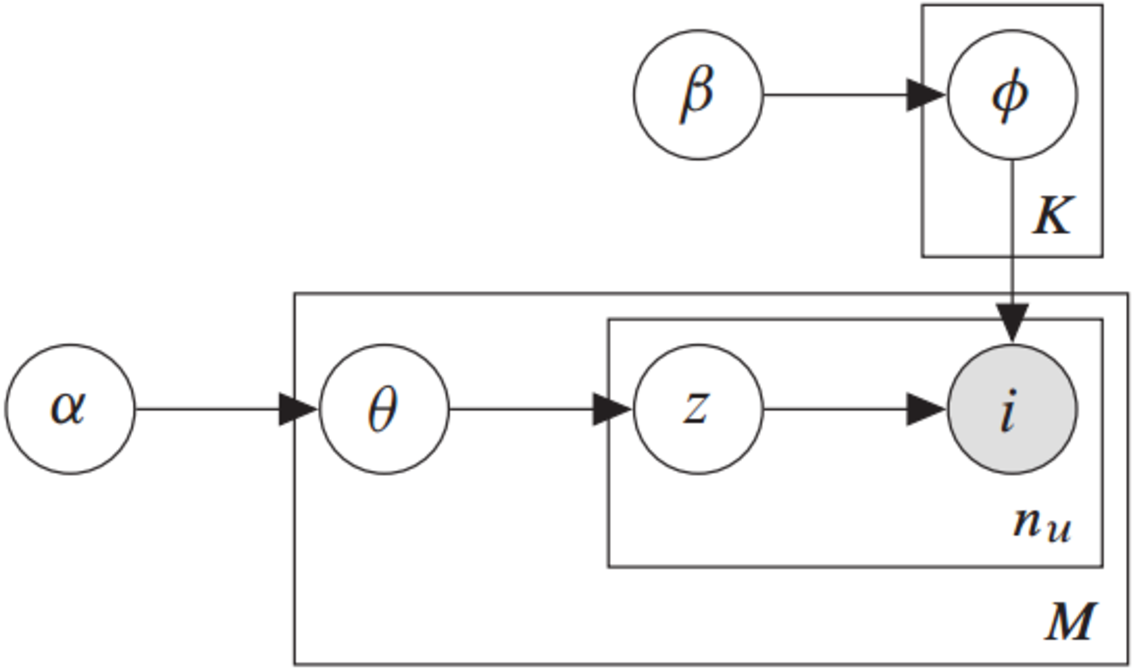
\includegraphics[width=0.4\textwidth]{Fig/bpmtmf/lda}	
% 	\caption{潜在狄利克雷分布}
% 	\label{fig-bpmtmf-lda}
% \end{figure*}
% 如图\ref{lda}所示,这个概率图可以分解为两个主要的物理过程:

% 1. $\alpha  \to \theta  \to z$ ,这个过程表示某一用户u的签到POI,首先由$\alpha$生成$\theta$,然后由$\theta$决定用户u第i个签到的POI的主题。

% 2. $\beta \to \phi \to i |k=z_{u,i}$ ,这个过程表示用如下方法生成用户u 第i个签到的POI:在$\Phi_1…\Phi_k$ 中,挑选$k=z_{u,i}$的,根据概率生成POI i。

% 联合分布如公式\ref{equ:pgm7}:
% \begin{equation}
% p(\vec{w},\vec{z}|\vec{\alpha},\vec{\beta})=p(\vec{w}|\vec{z},\vec{\beta})p(\vec{z}|\vec{\alpha})=\prod_{k=1}^{K}\frac{\Delta(\vec{n_k}+\vec{\beta})}{\Delta(\beta)}\prod_{m=1}^{M}\frac{\Delta(\vec{n_m}+\vec{\alpha})}{\Delta(\alpha)}
% \label{equ:pgm7}
% \end{equation}

% \section{多主题矩阵分解}

% \subsection{模型概览}
% n this paper, we assume that each user (or item) has different topic preference  and has a latent vector $\mathcal{P}_u^{h}\in \mathbb{R}^K$ (or $\mathcal{Q}_m^{h}\in \mathbb{R}^K$) for each topic $k$ instead of only one latent vector globally. As Figure \ref{fig:mamf} shows, we first divide data matrix into several submatrices.  Users (or items) in the same su-matrix are similar while users (or items) in the different submatrix do not have similar behavior. Then \textit{PBMF} is applied in each submatrix to get latent feature vectors for each topic. We propose a method called \textit{MTMF} under this idea. \textit{MTMF} combines traditional matrix factorization methods with topic modeling. Topic modeling specifies a co-occurrence data model which associates a latent factor with each single observation user-item pair $\langle u,i\rangle$. The generative process of \textit{MTMF} is as follows,
% \begin{itemize}
% 	\item[1.] For each user $u \in U$
% 	\begin{itemize}
% 		\item[(a)] Draw the number $n_u$ of item selections;
% 		\item[(b)] For each of the $n_u$ items to be generated;
% 		\begin{itemize}
% 			\item[i.] Draw a user topic $z_k\sim Disc(\theta_u)$
% 			\item[ii.] Draw the user latent factor $\mathcal{P}^{h}_u\sim \mathcal{N}(\mathcal{P}_u^{h}|0,\sigma_{\mathcal{P}^{h}}^2\mathbf{I})$ of topic $k$;
% 			\item[iii.] Draw an item $m\sim Disc(\phi_{z_k})$
% 			\item[iv.] Draw the item latent factor $\mathcal{Q}^{h}_m\sim \mathcal{N}(\mathcal{Q}_m^{h}|0,\sigma_{\mathcal{Q}^{h}}^2\mathbf{I})$ of topic $k$;
% 			\item[v.] Draw the rating $R_{um}\sim \mathcal{N}(\mathbf{R}_{um}|{\mathcal{P}_u^{h}}^\intercal\mathcal{Q}_m^{h},\sigma^2)$
% 		\end{itemize}
% 	\end{itemize}
% \end{itemize}
% So for user $u$ (or item), there are $K$ topic distribution value and $K$ latent feature vectors to model. Note that the topic model part can be replaced or extended by different probabilistic graphical models.

% The data likelihood function $P(\mathbf{R}|\Theta)$ for user-item matrix can be expressed as
% \begin{align}
% % \nonumber to remove numbering (before each equation)
% P(\mathbf{R}|\Theta)=&\prod_{\langle u,m\rangle}\sum_k^K\theta_{u,k}\phi_{k,m} \mathcal{N}(\mathbf{R}_{um}|{\mathcal{P}_u^{h}}^\intercal\mathcal{Q}_m^{h},\sigma^2)\nonumber \\
% & \mathcal{N}(\mathcal{P}_u^{h}|0,\sigma_{\mathcal{P}^{h}}^2\mathbf{I})\mathcal{N}(\mathcal{Q}_m^{h}|0,\sigma_{\mathcal{Q}^{h}}^2\mathbf{I}) \nonumber \\
% & \mathcal{N}(\mathbf{a}_u|0,\sigma^2_{\mathbf{a}}) \mathcal{N}(\mathbf{b}_m|0,\sigma^2_{\mathbf{b}})
% \end{align}
% where $\sum_{k}\theta_{u,k} = 1$ and $\sum_{m}\phi_{k,m} = 1$.

% In general, each prediction is estimated by the weighted sum of the topic ratings,
% \begin{align}
% \hat{R}_{um} = \frac{\sum_{k=1}^K\theta_{u,k}\phi_{k,m}({\mathcal{P}_u^{h}}^\intercal\mathcal{Q}_m^{h}+\mathbf{A}_u^{h}+\mathbf{B}_m^{h}+\mu)}{\sum_{k=1}^K\theta_{u,k}\phi_{k,m}}
% \end{align}
% We use global mean of observations in the training set as the predicted rating when $\sum_k^K\theta_{u,k}\phi_{k,m}=0$.

% \subsection{参数估计}
% \label{subsec:alg}
% We develop an Expectation Maximization algorithm  to learn the topics and latent feature vectors. By applying the EM framework, the complete data expectation log-likelihood of $\mathbf{R}$ given four regularization factors can be expressed as:
% \begin{align}
% &\mathbb{Q}(\Theta,\Theta') = \sum_{\langle u,m\rangle}\sum_k \gamma_{u,m,k}(\Theta')\{\log \theta_{k,u}+\log \phi_{m,k}-\nonumber \\
% & (\mathbf{R}_{um}-{\mathcal{P}_{u}^{h}}^\intercal\mathcal{Q}_{m}^{h}-\mathbf{A}_{u}^{h}-\mathbf{B}_{m}^{h}-\mu)^2
% -\lambda_{\mathcal{P}}{\mathcal{P}_{u}^{h}}^\intercal\mathcal{P}_{u}^{h} \nonumber \\
% &-\lambda_{\mathcal{Q}}{\mathcal{Q}_{m}^{h}}^\intercal\mathcal{Q}_{m}^{h}-\lambda_{\mathbf{A}}{\mathbf{A}_{u}^{h}}^2 -\lambda_{\mathbf{B}}{\mathbf{B}_{m}^{h}}^2 \}
% \end{align}

% We first use the \textit{PBMF} to initialize multi-topic user factors $\mathcal{P}$ and multi-topic item factors $\mathcal{Q}$. At first, we get topic distribution $\theta_u$ for user $u$ and  item distribution $\phi_k$ for topic $k$ by Equations (\ref{equ:gamma}), (\ref{equ:theta}) and (\ref{equ:phi}) while multi-topics latent factors are fixed.  Because different topics factors  $\mathcal{P}^{h}$ and $\mathcal{Q}^{h}$ are equal, it just equals \textit{PLSA} \cite{hofmann1999probabilistic} learning process. That is to say, we use \textit{PLSA} to initialize $\theta$ and $\phi$.
% Then we update topics and latent factors parameters together by \textit{EM} algorithm. In each iteration, \textit{SGD} (Stochastic Gradient Descent) is used for each topic matrix factorization by equations (\ref{equ:P}), (\ref{equ:Q}), (\ref{equ:A}) and (\ref{equ:B}).

% \begin{algorithm}[htp]
% 	\begin{algorithmic}[1]
% 		\caption{BPMTMF学习算法}
% 		\label{algo-pmtmf-learning}
% 		\REQUIRE{Set of data points $\mathcal{A}$, anchor number $H$, DCGASC function $f$ and sets $A^i$ covered by each data point $a_i$}
% 		\ENSURE{An anchor point order list $\hat{\mathcal{A}} \subseteq \mathcal{A}$ with $|\hat{\mathcal{A}}| = H$}
		
% 		\STATE {Use BPMF to initialize  $\mathbf{P}^{h}$ and  $\mathbf{Q}^{h}$;}
% 		\STATE {Use BPMF to initialize  $\mathbf{P}^{h}$ and  $\mathbf{Q}^{h}$;}
		
% 		\REPEAT 
		
% 		\FOR{each entry $i=\langle u,m\rangle$} 
% 		\STATE {Sample a topic assignment $z_i$ using Eq.~\ref{eq-bpmtmf-topic}:}
% 		\STATE {$$z_i=P(z_i=k|\mathbf{Z}_{\neg i},\mathbf{R},\mathbf{P},\mathbf{Q},\alpha,\beta,\sigma)$$}
% 		\ENDFOR
		
% 		\FOR{each topic $k=1,2,...,K$} 
		
% 		\STATE {Sample Gaussian-Wishart priors using Eq.~\ref{eq-bpmtmf-wishart}:}
% 		\STATE {$$\Psi_{\mathbf{P}}^{h}= P(\Psi_{\mathbf{P}}^{h}|\Psi_0^{h}), \ \Psi_{\mathbf{Q}}^{h}= P(\Psi_{\mathbf{Q}}^{h}|\Psi_0^{h})$$}
		
% 		\FOR{each user $u=1,2,...,N$} 
% 		\STATE {Sample users' topic-specific latent vectors using Eq.~\ref{eq-bpmtmf-usersGaussian}:}
% 		\STATE {$$\mathbf{P}^{h}_u=P(\mathbf{P}_u^{h}|\mathbf{R},\mathbf{Q}^{h},\Psi_{\mathbf{P}}^{h},\sigma_h)$$}
% 		\ENDFOR
		
% 		\FOR{each item $m=1,2,...,M$} 
% 		\STATE {Sample items' topic-specific latent vectors:}
% 		\STATE {$$\mathbf{Q}^{h}_m=P(\mathbf{Q}_u^{h}|\mathbf{R},\mathbf{P}^{h},\Psi_{\mathbf{Q}}^{h},\sigma_h)$$}
% 		\ENDFOR
		
% 		\ENDFOR	
		
% 		\UNTIL{Convergence}
		
% 	\end{algorithmic}
% \end{algorithm}

\section{贝叶斯多主题矩阵分解模型}
\label{sec-bpmtmf-model}
本章节主要介绍针对\textit{评分预测}的多主题矩阵分解模型的构建以及优化。 表\ref{tab-lwmf-notation}中列出了本章节中使用的符号表。基础的符号描述见表\ref{tab-basic-notation}中所示。矩阵和集合字符的小写上标,例如$\mathbf{R}^h$和$\mathcal{P}^h$,表示不同主题的子矩阵以及相应用户索引集合,这部分表示与第\ref{chapter-lwmf}章表示类似,只是每个子矩阵多了主题的概念。

\begin{table}
	\centering
	\caption{本章主要符号说明}
	\label{tab-bpmtmf-notation}%
	\begin{small}
		\begin{tabular}{cp{0.75\columnwidth}}
			\hline
			符号 & 符号描述 \bigstrut\\
			\hline\hline
			$\mathbf{R}^h$ & 第$h$个主题的子评分矩阵 \bigstrut\\
			$ \mathbf{V}^h$ & 第$h$个主题的子评分矩阵$\mathbf{R}^h$的权重矩阵\bigstrut\\
			$ \mathcal{P}^h$ & 第$h$个主题的用户索引集合  \bigstrut\\
			$ \mathcal{Q}^h$ & 第$h$个主题的商品索引集合  \bigstrut\\
			$ \mathbf{P}^h$  & 第$h$个主题的用户隐藏特征矩阵 \bigstrut\\
			$\mathbf{Q}^h$  &  第$h$个主题的商品隐藏特征矩阵 \bigstrut\\
			\hline
			$z_a$ ($z_{um}$)    &观察数据点$a=\langle u,m\rangle$上分配的主题\bigstrut \\
			$\theta_u$ & 第$u$个用户的主题分布($\in \mathbb{R}^H$) \bigstrut\\
			$\phi_h$ & 第$h$个主题上的商品分布($\in \mathbb{R}^M$) \bigstrut\\
			\hline
			$\alpha$ &主题模型上主题分布的狄利克雷先验参数\bigstrut \\
			$\beta$ &  主题模型上商品分布的狄利克雷先验参数\bigstrut\\
			$\Psi_0$ & 概率矩阵分解上高斯先验的高斯-维希特(Gaussian-Wishart)先验参数 \bigstrut\\
			\hline
		\end{tabular}%
	\end{small}
\end{table}%

\subsection{模型概览}
\label{subsec-bpmtmf-model}
本章节工作的主要思想是利用主题模型构造子矩阵聚类,然后利用多个特定主题的概率矩阵分解集成预测评分值。因此,本章节模型主要由两部分组成:
\begin{itemize}
	\item 对用户访问商品行为建模;
	\item 用户访问商品后,会对商品进行评分,对这一用户评分行为建模。
\end{itemize}

\subsubsection{对用户访问商品行为建模} 
为了对用户消费商品行为建模,本章工作采用一种类似文本文档聚类的标准主题模型的方法(例如,潜在狄利克雷分布~\cite{blei2003latent})做以下的类比:一个商品被认为是文档中的一个词,那么一个用户所评价过的商品集合作为一个文档。使用这种方法,一个\emph{主题}(\aka 商品主题)被定义为一个在商品集合上的多项式分布。本章工作让$\phi_h$表示为第$h$个主题,以及让$\phi_{hm}$表示第$h$个主题中生成第$m$个商品的概率。给定$H$个主题的集合,用户偏好则是这$H$个主题上的多项式分布。本章节让$\theta_u$表示第$u$个用户的主题分布,以及让$\theta_{uh}$表示第$u$个用户的主题分布上第$h$个主题概率。本章模型引入狄利克雷先验$Dir(\alpha)$和$Dir(\beta)$来分别生成多项式分布$\theta$和$\phi$,超参数分别为$\alpha$和$\beta$。主题建模一般用于产生用户访问过的商品集合,如下表示:

\begin{equation}
\label{eq-bpmtmf-topicmodel}
p(\{\langle u,m\rangle\}) \propto \prod_{\langle u,m\rangle} \bigg( \sum_{h} \theta_{uh}\phi_{hm} \bigg),
\end{equation}
其中$\langle u,m\rangle$数据点对表示第$u$个用户已经访问过第$m$个商品。公式~\ref{eq-bpmtmf-topicmodel}列举了训练数据集中所有的$\langle u,m\rangle$数据点对。

\subsubsection{对用户评分行为建模} 
为了对用户评分行为建模,主题被认为是上下文信息,更进一步地说,一个用户或者商品在每个主题上会有一个主题相关的隐藏特征向量与之相对应。本章节让$\mathbf{P}_u^{h}\in \mathbb{R}^K$ (或者 $\mathbf{Q}_m^{h}\in \mathbb{R}^K$)表示第$u$个用户(或者$m$第个商品)第$h$个主题对应的主题特定的隐藏特征向量。本章模型假设,每个用户将在不同主题上下文信息下表现出不同评分偏好,以及每个商品也将会在不同主题上下文信息下显示出不同的被评分模式。举个例子,如果一个用户是星球大战粉丝,那么相对于其他动作电影来说,这个用户可能会对``星球大战"系列电影打出较高的分数。这里需要注意,简单地融合目录偏差,如论文~\cite{mirbakhsh2013clustering,hu2014your} 所示,是不适用于上述例子的,因为用户在``动作"类影片中既可能打高分也有可能标记为低分。融合目录偏差,比较适用于以下情形,例如,儿童用户更喜欢``动漫"类电影,而理解不了``人性"类电影从而打低分。而本章模型尝试去建模用户评分行为时主题上下文对个人因素的影响。这样就能保证本章模型能够适用于以上两种,甚至更多的情形。为了获得特定主题的隐藏特征向量,本章采用在隐藏特征向量$\mathbf{P}^{h}$和$\mathbf{Q}^{h}$上使用高斯-维希特(Gaussian-Wishart)先验参数,对应的超参数有$\Psi_{\mathbf{P}}^{h}=\{\mu_{\mathbf{P}}^{h}, \Lambda_{\mathbf{P}}^{h}\}$和$\Psi_{\mathbf{Q}}^{h}=\{\mu_{\mathbf{Q}}^{h}, \Lambda_{\mathbf{Q}}^{h}\}$,具体公式如下表示:

\begin{equation}
	\label{eq-bpmtmf-wishart}
	p(\Psi^{h}|\Psi_0^{(h)}) = \mathcal{N}(\mu^{(h)}|\mu_0^{h},(\xi_0^{h} \Lambda^{h})^{-1})\mathcal{L}(\Lambda^{h}|\mathbf{L}_0^{h},\nu_0^{h})
\end{equation}
其中$\nu_0^{h}$是Wishart分布$\mathcal{L}^{h}$自由度参数,$\mathbf{L}_0^{h}$是规模矩阵(对于用户,$\mathbf{L}_0^{h}\in \mathbb{R}^{N\times N}$;对于商品,$\mathbf{L}_0^{h}\in \mathbb{R}^{M\times M}$ ),$\Psi_0^{h} = \{\mu_0^{h},\nu_0^{h},\mathbf{L}_0^{h}\}$则是所有第$k$个主题对应的参数。类似于文章~\cite{salakhutdinov2008bayesian}所示,如上先验参数,则是由如下公式生成:

\begin{align*}
&{\mu_0^{h}}^\ast = \frac{\beta_0 \mu_0+N^{h} \bar{\mathbf{P}}^{h}}{\beta_0+N^{h}},\ \ {\beta_0^{h}}^\ast = \beta_0+N^{h},\ \ {\nu_0^{h}}^\ast = \nu_0+N^{h}\\
& [{\mathbf{L}_0^{h}}^\ast]^{-1} = \mathbf{L}_0^{-1}+N^{h}\bar{S}^{h}+\frac{\beta_0N^{h}}{\beta_0+N^{h}}(\mu_0-\bar{\mathbf{P}}^{h})(\mu_0-\bar{\mathbf{P}}^{h})^\mathrm{ T }\\
&\bar{\mathbf{P}}^{h}=\frac{1}{N^{h}}\sum_{u\in U^{h}}\mathbf{P}_u^{h},\ \ \bar{S}=\frac{1}{N^{h}}(\mathbf{P}_u^{h}-\bar{\mathbf{P}}^{h})(\mathbf{P}_u^{h}-\bar{\mathbf{P}}^{h})^\mathrm{ T }
\end{align*}


因此,给定第$k$个主题,利用高斯-维希特(Gaussian-Wishart)公式~\ref{eq-bpmtmf-wishart}得到先验参数进而计算特定主题的用户隐藏特征向量$\mathbf{P}^{h}$和商品隐藏特征向量$\mathbf{Q}^{h}$,可以根据高斯分布计算出该主题下的第$u$个用户对第$m$个商品的评分值:

\begin{equation}
\label{eq-bpmtmf-ratingmodel}
p(\mathbf{R}_{um}|\mathbf{P}_u^{h},\mathbf{Q}_m^{h},\sigma_h^2)=\mathcal{N}(\mathbf{R}_{um}|{\mathbf{P}_{u}^{h}}^{\top} \mathbf{Q}_{m}^{h},\sigma_h^2),
\end{equation}
其中${\mathbf{P}_{u}^{h}}^{\top} \mathbf{Q}_{m}^{h}$为高斯分布均值,$\sigma_h^2$是高斯分布的方差。

\subsubsection{最终模型} 
本章提出的模型,称为贝叶斯概率多主题矩阵分解模型(Bayesian Probabilistic Multi-Topic Matrix Factorization,简称BPMTMF),融合了两个组件,也就是对用户消费商品行为建模(公式~\ref{eq-bpmtmf-topicmodel})和对评分建模(公式~\ref{eq-bpmtmf-ratingmodel}),使用了全贝叶斯的方法。图~\ref{fig-bpmtmf-generativeprocess}展示了BPMTMF的生成过程。生成过程可以如下描述。当第$u$个用户想要对第$m$个商品进行评分时,用户首先需要根据她的主题分布$\theta_u$选择第$h$个主题$z$,然后由该主题$z$的商品分布生成第$m$个商品。最后,评分是基于第$h$个主题$z$的用户隐藏特征向量$\mathbf{P}_{u}^{h}$和商品隐藏特征向量$\mathbf{Q}_{m}^{h}$生成,该评分分布符合高斯分布。因此,给定参数,对于所有的评分的似然函数如下表示:

 \begin{align}
	\label{eq-bpmtmf-obj}
	p(\mathbf{R}|\alpha,\beta, \Psi_0,\sigma)=&\\
	\int &\big(\prod_u P(\theta_u|\alpha)\big)\big(\prod_h P(\phi_h|\beta)P(\Psi_{\mathbf{P}}^{h}|\Psi_0^{h})P(\Psi_{\mathbf{Q}}^{h}|\Psi_0^{h})\big)\nonumber\\
	&\big(\prod_h \prod_m P(\mathbf{Q}_m^{h}|\Psi_{\mathbf{Q}}^{h})\big)\big(\prod_k \prod_u P(\mathbf{P}_u^{h}|\Psi_{\mathbf{P}}^{h})\big)\nonumber\\
	&\big(\prod_{\langle u,m\rangle}\sum_{h} \theta_{uh}\cdot \phi_{hm}\cdot P(\mathbf{R}_{um}|\mathbf{P}_u^{h},\mathbf{Q}_m^{h}, \sigma_h^2)\big)\nonumber\\
	&\mathrm{d}\mathbf{P}_u^{h}\mathrm{d}\mathbf{Q}_m^{h}\mathrm{d}\Psi_{\mathbf{P}}^{h}\mathrm{d}\Psi_{\mathbf{Q}}^{h}\mathrm{d}\theta_u \mathrm{d}\phi_h.\nonumber
	\end{align}

值得注意地是,设置特定主题的隐藏特征向量将会随着优化而造成过拟合,然而本章的贝叶斯方法通过先验参数可以有效地控制模型的复杂度。尽管本章模型融合了更多的超参数,在模型BPMF~\cite{salakhutdinov2008bayesian}以及之后的实验结果表明,模型性能相对来说对参数的取值不敏感。


\begin{figure}
	\centering
		\begin{itemize}
			\item[1.] 对每一个主题$h=1,...,H$,
			\begin{itemize}
				\item[(1)] 抽样一个多项式主题分布$\phi_h \sim Dir(\beta)$
				\item[(2)] 抽样特定主题的用户隐藏特征向量和商品隐藏特征向量的超参数$p(\Psi_{\mathbf{P}}^{h}|\Psi_0^{h})$ 和$p(\Psi_{\mathbf{Q}}^{h}|\Psi_0^{h})$
			\end{itemize}
			\item[2.] 对每一个商品$m=1,...,M$,
			\begin{itemize}
				\item[i.] 对每个主题$h=1,...,H$,抽样特定主题的商品隐藏特征向量${\mathbf{Q}_{m}^{h}} \sim p(\mathbf{Q}_{m}^{h}|\Psi_{\mathbf{Q}}^{h})$	 	
			\end{itemize}
			\item[3.] 对每一个用户$u=1,...,N$,
			\begin{itemize}
				\item[i.] 抽样$\theta_u \sim Dir(\alpha)$
				\item[ii.] 对每一个主题$h=1,...,H$,抽样特定主题的用户隐藏特征向量${\mathbf{P}_{u}^{h}} \sim p(\mathbf{P}_{u}^{h}|\Psi_{\mathbf{P}}^{h})$
				\item[iii.] 对每个被第$u$个用户评分的商品(第$m$个商品)
				\begin{itemize}
					\item[(1)] 抽样一个主题$z\sim Disc(\theta_u)$(第$h$个主题)
					\item[(2)] 从第$h$个主题中抽样第$m$个商品,$m\sim Disc(\phi_{z})$
					\item[(3)] 根据高斯分布抽样评分,$\mathbf{R}_{um}\sim \mathcal{N}(\mathbf{R}_{um}|{\mathbf{P}_{u}^{h}}^\top \mathbf{Q}_{m}^{h},\sigma_h^2)$
				\end{itemize}
			\end{itemize}
		\end{itemize}
	\caption{BPMTMF模型生成过程}
	\label{fig-bpmtmf-generativeprocess}
\end{figure}


\subsection{吉布斯采样参数学习}
\label{subsec-bpmtmf-gibbs}
在本章节模型中,需要学习的参数(或者变量)如下列出:
\begin{itemize}
	\item[(1)] $\{\theta_u\}$,用户主题分布;
	\item[(2)] $\{\phi_h\}$,主题商品分布;
	\item[(3)] $\{\mathbf{P}_u^{h}\}$ ,第$h$个主题的用户隐藏特征向量,$h=1,...,H$;
	\item[(4)] $\{\mathbf{Q}_m^{h}\}$,第$h$个主题的商品隐藏特征向量,$h=1,...,H$;
\end{itemize}

本小节的工作就是去学习这些参数$\{\theta,\phi, \mathbf{P}, \mathbf{Q}\}$,以至于可以最大化观察评分矩阵$\mathbf{R}$的似然函数。因为参数的复杂性和隐藏变量等因素的存在,去直接优化该目标函数显得非常困难。因此,在推理和参数学习上本章节工作将采用广泛使用的Gibbs采样算法进行优化。在每轮迭代中,本章节工作相互迭代学习主题分布,更新特定主题的用户隐藏特征向量$\{\mathbf{P}_u^{h}\}$和商品隐藏特征向量$\{\mathbf{Q}_m^{h}\}$。当算法达到收敛时,本章节工作将使用各个数据点的主题选择来估计用户主题分布变量$\{\theta_u\}$和主题商品分布变量$\{\phi_h\}$。

\subsubsection{推断主题分布}
固定所有其他特定主题的隐藏特征向量和超参数,对数据点$a=\langle u,m\rangle$能够得到以下条件概率分布:

\begin{align}
	\label{eq-bpmtmf-topic}
	p(z_a=&h|\mathbf{Z}_{\neg a},\mathbf{R},\mathbf{P},\mathbf{Q},\alpha,\beta,\sigma)  \\\nonumber
	\propto&\frac{n_{u}^h+\alpha-1}{\sum_{j=1}^H (n_{u}^j+\alpha)-1}\times\frac{n_{m}^h+\beta-1}{\sum_{m'=1}^{M}(n_{m'}^{h}+\beta)-1}\times\mathcal{N}(\mathbf{R}_{um}|{\mathbf{P}_{u}^{h}}^{\top}\mathbf{Q}_{m}^{h},\sigma_h^2),\nonumber
\end{align}
其中$n_{u}^h$表示第$u$个用户的评分商品中属于第$h$个主题的商品的个数,$n_{m}^h$ 代表那些在第$m$个商品评过分且属于第$h$个主题的用户个数,以及评分值$\mathbf{R}_{um}$是通过在第$h$个主题上利用该主题的隐藏特征向量,使用高斯分布$\mathcal{N}(\mathbf{R}_{um}|{\mathbf{P}_{u}^{h}}^{\top}\mathbf{Q}_{m}^{h},\sigma_h^2)$产生的。实际上,该采样公式类似于原始LDA模型的Gibbs优化公式~\cite{heinrich2005parameter},只是在该公式的基础上本章工作加入了评分产生的公式项。

\subsubsection{更新特定主题的隐藏特征向量}
更新特定主题的用户和商品隐藏特征向量跟原始的贝叶斯概率矩阵分解(BPMF)~\cite{salakhutdinov2008bayesian}非常相似。两者不同之处是,本章工作假设每个被评分的商品的主题是给定的,因此每个特定主题的用户商品隐藏特征向量的更新跟特定主题的用户和商品有关。这里,特定主题的用户隐藏特征向量$\mathbf{P}_u^{h}$的条件概率服从高斯分布:

\begin{align}
\label{eq-bpmtmf-usersGaussian}
p(\mathbf{P}_u^{h}|\mathbf{R},\mathbf{Q}^{h},\Psi_{\mathbf{P}}^{h},\sigma_h^2) =&\ \mathcal{N}(\mathbf{P}_u^{h}|{\mu_{\mathbf{P}}^{h}}^*,[{\Lambda_{\mathbf{P}}^{h}}^*]^{-1}) \\\nonumber
\propto&\ P(\mathbf{P}_u^{h}|\mu_{\mathbf{P}}^{h},\Lambda_{\mathbf{P}}^{h})\prod_{m=1 }^M\mathcal{N}(\mathbf{R}_{um}|{\mathbf{P}_u^{h}}^{\top} \mathbf{Q}_m^{h},\sigma_h^2)^{\mathbf{I}^{h}_{um}}\nonumber
\end{align}
这里原始高斯分布的均值和方差如下公式计算:

\begin{align}
&{\Lambda_u^{h}}^\ast =\Lambda_{\mathbf{P}^{h}}+\frac{1}{\sigma_h^2}\sum_{m=1}^M(\mathbf{Q}_m^{h}{\mathbf{Q}_m^{h}}^{\top})^{\mathbf{I}^{h}_{um}} \label{eq-bpmtmf-var}\\
&{\mu_u^{h}}^\ast = [{\Lambda_u^{h}}^*]^{-1}(\Lambda_{\mathbf{P}^{h}}\mu_{\mathbf{P}^{h}}+\frac{1}{\sigma_h^2}\sum_{m=1}^M(\mathbf{Q}_m^{h} \mathbf{R}_{um}))^{\mathbf{I}^{h}_{um}}\label{eq-bpmtmf-mean}
\end{align}
其中$\mathbf{I}^{h}_{um}$是指示标识值,当主题分布符合$z_{um}=h$时,值为1,其他情况则为0,即不将其考虑在参数学习内。同理,本章工作使用相似的公式计算特定主题的商品隐藏特征向量$\{\mathbf{Q}_m^{h}\}$,这里省略描述。

 \begin{algorithm}
 	
	\begin{algorithmic}[1]
		\caption{BPMTMF学习算法}
		\label{algo-bpmtmf-learning}
		\REQUIRE{评分矩阵$\mathbf{R}$,主题个数$H$,用户和商品隐藏特征向量维度$K$;}
		
		\STATE {使用BPMF得到的全局用户和商品隐藏特征向量初始化各个局部隐藏特征向量$\mathbf{P}^{h}$ 和$\mathbf{Q}^{h}$;}
		\STATE {使用LDA的主题分布初始化BPMTMF中的主题分布;}

		
		\REPEAT 
		
		\FOR{每一个数据点$a=\langle u,m\rangle$} 
			\STATE {利用公式~\ref{eq-bpmtmf-topic}对数据点$a$分配主题$z_a$:}
			\STATE {$$z=p(z=h|\mathbf{Z}_{\neg a},\mathbf{R},\mathbf{P},\mathbf{Q},\alpha,\beta,\sigma)$$}
		\ENDFOR
		
		\FOR{每个主题$h=1,2,...,H$} 
		
			\STATE {根据公式~\ref{eq-bpmtmf-wishart}采样高斯-维希特(Gaussian-Wishart)先验参数:}
			\STATE {$$\Psi_{\mathbf{P}}^{h}= P(\Psi_{\mathbf{P}}^{h}|\Psi_0^{h}),$$
				$$\Psi_{\mathbf{Q}}^{h}= P(\Psi_{\mathbf{Q}}^{h}|\Psi_0^{h})$$}
			
			\FOR{每个用户$u=1,2,...,N$} 
				\STATE {根据公式~\ref{eq-bpmtmf-usersGaussian}采样用户主题特定的隐藏特征向量:}
				\STATE {$$\mathbf{P}^{h}_u=P(\mathbf{P}_u^{h}|\mathbf{R},\mathbf{Q}^{h},\Psi_{\mathbf{P}}^{h},\sigma_h)$$}
			\ENDFOR
			
			\FOR{每个商品$m=1,2,...,M$} 
				\STATE {采用商品主题特定的隐藏特征向量:}
				\STATE {$$\mathbf{Q}^{h}_m=P(\mathbf{Q}_u^{h}|\mathbf{R},\mathbf{P}^{h},\Psi_{\mathbf{Q}}^{h},\sigma_h)$$}
			\ENDFOR
			
		\ENDFOR	

		\UNTIL{收敛}
		
	\end{algorithmic}
\end{algorithm}

\subsubsection{整体学习算法}
算法~\ref{algo-bpmtmf-learning}描述本章BPMTMF模型学习参数的Gibbs采样算法~\cite{andrieu2003introduction}。在最开始,本章工作使用BPMF得到全局的用户隐藏特征向量$\mathbf{P}$和商品隐藏特征向量$\mathbf{Q}$,去初始化$H$个特定主题的用户隐藏特征向量$\mathbf{P}^{h}$和商品隐藏特征向量$\mathbf{Q}^{h}$。对于数据点主题分布,本章工作使用标准的LDA(不考虑评分的情况下)进行初始化训练集中数据点主题分布。在每轮迭代,本章模型首先对所有可观察到的训练集数据点进行抽样,分配主题,然后固定数据点的主题分布更新特定主题的用户隐藏特征向量$\mathbf{P}^{h}$和商品隐藏特征向量$\mathbf{Q}^{h}$。过了初始时间阶段,本章工作将通过简单的计算方法估计每迭代一轮后的用户主题分布参数$\{\theta_u\}$和主题商品分布参数$\{\phi_h\}$ ,公式如下:

\begin{align}
	\label{eq-bpmtmf-topicpara}
	\theta_{uh} = \frac{n_{u}^h+\alpha}{\sum_{j=1}^H (n_{u}^j+\alpha)},\ 
	\phi_{hm} = \frac{n_{m}^h+\beta}{\sum_{m'=1}^{M}(n_{m'}^h+\beta)}
\end{align}
其中$n_{u}^h$,$n_{u}^h$,$n_{m}^h$和$n_{h}^h$是在公式~\ref{eq-bpmtmf-topic}中的各类计数。

\subsubsection{计算复杂度分析} 
本小节中符号$|\mathbf{R}|$表示数据矩阵$\mathbf{R}$的非零观察值的个数,以及$n_{u,\cdot}^h=\sum_{m}\mathbf{I}^{h}_{um}$代表第$u$个用户的第$h$个主题中评过分的商品个数。在每一轮迭代中,更新主题分配任务中,总共需要采样$|\mathbf{R}|$次,每次样本点根据公式~\ref{eq-bpmtmf-topic}需要计算$H$次概率,且每次概率计算(公式~\ref{eq-bpmtmf-topic})因为加入了评分项计算,复杂度为$O(K)$,所以更新整个主题分配的复杂度为$\mathcal{O}(HKS)$。对于更新用户的隐藏特征向量,主要的计算花费在公式~\ref{eq-bpmtmf-var}上$\sum_{m=1}^M(\mathbf{Q}_m^{h}{\mathbf{Q}_m^{h}}^{\top})^{\mathbf{I}^{h}_{um}}$计算均值部分以及公式~\ref{eq-bpmtmf-mean}计算方差的矩阵逆计算项${\Lambda_u^{h}}^*$,对应的复杂度分别为$\mathcal{O}(K^2n_{u,\cdot}^{h})$和$\mathcal{O}(K^3)$。这里类似于文章~\cite{hu2008collaborative},尽管有更高效的算法存在,本小节假设计算大小为$\mathbb{R}^{K \times K }$的矩阵的逆所需要的时间复杂度为$\mathcal{O}(K^3)$。因此,更新均值${\Lambda_u^{h}}^\ast$和方差${\mu_u^{h}}^\ast$的时间复杂度为$\mathcal{O}(K^3+K ^2n_{u,\cdot}^{h})$。并且,优化算法还需要遍历$N$个用户和$H$个主题,这将会导致整个更新隐藏特征向量迭代复杂度变为$\mathcal{O}(K^3HN+K^2|\mathbf{R}|)$,其中$|\mathbf{R}|=\sum_{u,k}n_{u,\cdot}^h$。同理,更新全部商品的各个主题的隐藏特征向量的时间复杂度为$\mathcal{O}(K^3HM+K^2|\mathbf{R}|)$。综合以上所有部分,每一轮迭代本文模型BPMTMF的时间复杂度为$\mathcal{O}(KH|\mathbf{R}|+K^2|\mathbf{R}|+K^3HN+K^3HM)$。可以看出,总的算法复杂度跟数据集大小成正比,跟用户个数和商品个数成正比,跟主题个数成正比,跟隐藏特征向量维度的三次成正比。因为隐藏特征向量维度和主题个数一般不会太大,模型的时间复杂度跟数据集大小成正比是比较容易接受的。


\subsection{评分预测}
\label{subsec-bpmtmf-prediction}
当所有BPMTMF的参数都学习优化完之后,本章工作将使用以下公式进行最终的用户商品评分预测:

\begin{equation}\label{eq-bpmtmf-finalpred}
	\hat{\mathbf{R}}_{um} \approx 
	\frac{1}{\sum_{h'=1}^{H}\theta_{uh'}\cdot \phi_{mh'}}\sum_{h=1}^{H} \bigg\{(\theta_{uh}\cdot\phi_{mh}) ({\mathbf{P}_u^{h}}^{\top} \mathbf{Q}_m^{h})\bigg\},\nonumber
\end{equation}
其中$\hat{\mathbf{R}}_{um}$是$\mathbf{R}_{um}$的预测评分,其实就是用户商品在各个主题的加权平均预测值。需要注意的是,上述预测评分公式仅仅只用了一轮的Gibbs采样值,在多轮采样上则需要对每轮预测值进行简单平均。

\subsubsection{与相关工作的联系} 
公式~\ref{eq-bpmtmf-localmf}展示了之前在非概率局部矩阵分解上相关工作的一般数学形式~\cite{MJT11,lee2013local,chen2015wemarec}。值得注意的是,本章模型的预测公式~\ref{eq-bpmtmf-finalpred}和公式~\ref{eq-bpmtmf-localmf}有非常紧密的联系。给定一组用户-商品对数据点$a=\langle u,m\rangle$,本章工作可以有相似的对应关系:${\mathbf{P}_u^{h}}^{\top}\mathbf{Q}_m^{h}\rightarrow \hat{\mathbf{R}}_{um}^{h}$代表的是在第$h$个``聚类"中数据点$\mathbf{R}_{um}$的预测评分,$\theta_{uh}\cdot\phi_{hm}\rightarrow \mathbf{L}_{um}^{h}$则是代表第$h$个``聚类"中该商品-用户对数据点的预测值$\hat{\mathbf{R}}_{um}^{h}$,以及$\sum_{h'=1}^{H}\theta_{uh'}\cdot \phi_{h'm}\rightarrow \mathbf{Z}_{um}$则扮演了归一化系数的角色。诸如此类的类比表明,本章模型形式可以被看作是之前非概率局部矩阵分解的概率版本:在公式~\ref{eq-bpmtmf-localmf}中一个聚类在本文BPMTMF模型中则代表的是一个主题。如此紧密的联系使得之前的非概率局部矩阵分解相关工作能够以概率的形式所解释,进而可以有更深入的理论分析和扩展。

\section{实验及分析}
\label{sec-bpmtmf-experiments}
本节将在真实显式评分数据上评估本章提出的模型。本章节首先介绍实验所使用的真实世界数据集、评价指标、对比方法以及参数设置。随后实验分析\textit{评分预测}的模型性能,对比聚类结果以及主题个数对推荐效果和模型训练时间的影响。
\subsection{实验设置}
\subsubsection{数据集说明}
实验将在两个公共的、广泛作为标准数据集使用的电影数据上验证本章提出的BPMTMF模型。一个是 Movielens数据集\footnote{\url{http://www.grouplens.org/}},另一个是Netflix数据集\footnote{\url{http://www.netflixprize.com/}}(2007年,Netflix百万美元奖金竞赛的数据集)。两个数据集的具体描述如表~\ref{tab-bpmtmf-data}所示。实验随机将整个数据集以$9:1$的比例切分为训练集和测试集。最后取5次以相同方式随机切分得到的数据集的模型预测作为最终推荐结果。

\begin{table}
	\centering
	\caption{显示评分数据集Movielens和Netflix的详细信息}
	\label{tab-bpmtmf-data}%

		\begin{tabular}{c||cccc}
			\hline
			数据集 & \#用户 & \#商品 & \#评分 & 稠密度 \bigstrut\\
			\hline
			\hline
			Movielens &  69,878 &  10,677 & 10,000,054 & 1.31\% \bigstrut\\
			Netflix & 480,189 & 17,770 & 100,000,000 & 1.17\% \bigstrut\\
			\hline
		\end{tabular}%

\end{table}%

\subsubsection{评价指标}
本实验采用两个常用的评价指标去评价预测正确率,均方根误差(Root Mean Square Error, RMSE)和平均绝对误差(Mean Absolute Error, MAE),如下公式定义:

\begin{align}
	RMSE &= \sqrt{\frac{\sum_{\langle u,m\rangle}(\mathbf{R}_{um}-\hat{\mathbf{R}}_{um})^2}{n_{test}}}
\end{align}
其中$n_{test}$指的是测试集中有评分值的数据点数量。更小的RMSE和MAE代表了更好的性能。
%	MAE &= \frac{|\mathbf{R}_{um}-\hat{\mathbf{R}}_{um}|}{N_{test}}
\subsubsection{对比方法}
本实验将本章提出的BPMTMF模型与以下基线方法进行对比:

\begin{itemize}
	\item DFC~\cite{MJT11}:  该模型将大规模矩阵分解任务随机分解成更小的子问题,其中每个子矩阵中的数据没有一定的相关性,然后用均值组合子矩阵预测值来近似原始矩阵。
	\item LLORMA~\cite{lee2013local}\footnote{代码:\url{http://prea.gatech.edu/download.html\#ver20},Ver2.0版本}: 该方法从训练集中随机选择数个数据点作为锚点集合,然后根据每个锚点利用非参核函数选择与该锚点相关的训练数据点组成子矩阵,从而保证每个子矩阵具有局部相关性质,最后对每个子矩阵进行奇异值分解后利用公式~\ref{eq-bpmtmf-localmf}进行加权平均聚合成原始近似矩阵。
	\item WEMAREC~\cite{chen2015wemarec}\footnote{代码:\url{https://github.com/ldscc/StableMA}}: 该方法利用分段联合聚类对训练数据集聚类,每个聚类作为一个子矩阵,然后提出一种基于子矩阵的权重策略来预测用户对商品的评分。
	\item PMTMF: 对贝叶斯版局部矩阵分解的直接比较,本章节也实现了非贝叶斯版的概率多主题矩阵分解模型,没有先验超参数,使用极大似然估计和期望最大化算法(Expectation-Maximization, EM算法)优化主题分布部分,使用随机梯度下降优化特定主题的隐藏特征向量学习部分。
\end{itemize}

因为之前的研究~\cite{MJT11,lee2013local,chen2015wemarec}已经展示了上述基于局部的矩阵分解模型推荐性能优于传统方法,本实验中不再使用传统的矩阵分解~\cite{MS07,koren2009matrix} 作为基线方法进行比较。本实验在Java推荐系统开源工具librec~\cite{guo2015librec}上实现了本文的两个局部矩阵分解模型PMTMF和BPMTMF。

\subsubsection{参数设置} 
跟随论文~\cite{chen2015wemarec,lee2013local}参数的设置,对于所有局部矩阵分解模型,隐藏特征向量的维度$D$设置为$20$。对于本章模型PMTMF和BPMTMF,根据经验设置模型主题个数$H$为20;跟随论文~\cite{griffiths2004finding}超参数设置,用户主题分布狄利克雷超参数$\alpha$设置为$\frac{50}{H}$,主题商品分布狄利克雷超参数$\beta$设置为$0.01$;对于特定主题的隐藏特征向量部分的超参数设置,本实验跟随论文BPMF~\cite{salakhutdinov2008bayesian}的超参数设置,初始化$\mu_0^{h}=0$,\ $\nu_0^{h} = D$, $\mathbf{L}_0^{h}$为单位矩阵以及方差$\sigma_h^2=2$。由论文~\cite{salakhutdinov2008bayesian}的实验结果可以发现,当BPMF的迭代轮数超过150轮时,该模型的推荐准确率已经达到一个相对平衡的状态。因此,对于本文贝叶斯版本的概率主题模型,本实验首先用200轮的主题分布模型和100轮的隐藏特征向量学习来初始化,之后又进行了150轮的相互迭代进行最终模型参数的学习。因为实验中有相似的实验设置和相同的数据集,基线方法的其他参数设置为原始论文给出的最优参数数值。

\subsection{实验结果及分析}

\subsubsection{评分预测性能比较}
\label{subsec-bpmtmf-compare}
表~\ref{tab-bpmtmf-rmse}展示了各类评分预测模型的预测评分性能。在所有基线方法中,最近提出的局部矩阵分解模型WEAREC性能最好。WEMAREC采用了分段联合聚类方法来生成子矩阵,代表了当前局部矩阵分解模型的预测评分性能水平。同时,本小节实验也检验了本章提出的模型PMTMF和BPMTMF的性能。实验中能够发现非贝叶斯版的概率多主题矩阵分解的推荐准确率仅仅比最好的基线方法WEMAREC差一点点。并且,可以看出贝叶斯版BPMTMF比PMTMF和WEMAREC预测准确率都有很大提升,同时也证明了全贝叶斯方法的有效性。因此,BPMTMF比PMTMF推荐准确率高的很重要的一个原因是因为贝叶斯模型能够更加有效地控制模型的复杂度。对比这些基线方法,BPMTMF提供了一种更有原则性的解决方案,去融合子矩阵生成和权重选择。 得益于贝叶斯方法中先验超参数的存在,实验中需要更少的经验去设置参数同时得到较好的推荐效果。作为比较,WEMAREC需要首先去设置联合聚类的一系列参数,并且在融合权重的时候需要注意更多的相关参数设置。

\begin{table}
	\centering
	\caption{不同方法的RMSE结果对比}

		\begin{tabular}{|c||c|c|}
			\hline
			方法     & MovieLens & Netflix \bigstrut\\
			\hline
			\hline
			DFC   & 0.8064 & 0.8451 \bigstrut\\
			\hline
			LLORMA & 0.7834 & 0.8243 \bigstrut\\
			\hline
			WEMAREC & 0.7769 & 0.8142 \bigstrut\\
			\hline
			\hline
			PMTMF & 0.7792 & 0.8198 \bigstrut\\
			\hline
			\textbf{BPMTMF} & \textbf{0.7679} & \textbf{0.8081} \bigstrut\\
			\hline
		\end{tabular}%

	\label{tab-bpmtmf-rmse}%
\end{table}%

\subsubsection{聚类分析}
\label{subsec-bpmtmf-cluster} 
\begin{table*}
	\centering
	\caption{Movielens数据集上采样的两个主题或聚类的前10个流行电影。符号勾代表了相关电影在合适的目录}
	\label{tab-bpmtmf-cluster}%
	
	\subtable[动作片]{
	\begin{tabular}{|c||p{6cm}|p{6cm}|}
	\hline
		        序号 &     LLORMA &     BPMTMF \bigstrut\\
		\hline
		\hline
		         1 &  $\surd$ 星球大战4之新希望 & $\surd$ 夺宝奇兵3之圣战骑兵 \bigstrut\\
		\hline
		         2 & $\surd$ 星球大战5之帝国反击战 &   $\surd$    夺宝奇兵 \bigstrut\\
		\hline
		         3 & $\times$      美国丽人 &    $\surd$   虎胆龙威 \bigstrut\\
		\hline
		         4 &  $\times$     莎翁情史 &  $\surd$ 星球大战4之新希望 \bigstrut\\
		\hline
		         5 &    $\surd$  拯救大兵瑞恩 &       $\surd$  终结者 \bigstrut\\
		\hline
		         6 &    $\times$    外星人E.T. & $\surd$ 星球大战5之帝国反击战 \bigstrut\\
		\hline
		         7 &    $\times$       傀儡人生 &      $\surd$  蝙蝠侠 \bigstrut\\
		\hline
		         8 &     $\times$       第六感 &$\surd$ 星球大战6之绝地归来 \bigstrut\\
		\hline
		         9 &    $\surd$    黑衣人 &$\surd$ 夺宝奇兵2之魔域奇兵 \bigstrut\\
		\hline
		        10 &$\surd$ 星球大战6之绝地归来 & $\surd$   猎杀红色十月号 \bigstrut\\
		\hline
	\end{tabular}
	}\\
	$\ $\\
	\hspace{0.5cm}\\
	\subtable[剧情片]{
	\begin{tabular}{|c||p{6cm}|p{6cm}|}
		\hline
		        序号 &     LLORMA & $\surd$    BPMTMF \bigstrut\\
		\hline
		\hline
		         1 &    $\surd$   美国丽人 &  $\surd$    沉默的羔羊 \bigstrut\\
		\hline
		         2 &   $\surd$    勇敢的心 &  $\surd$   拯救大兵瑞恩 \bigstrut\\
		\hline
		         3 &  $\surd$   拯救大兵瑞恩 &  $\surd$   肖申克的救赎 \bigstrut\\
		\hline
		         4 &     $\times$      洛城机密 &   $\surd$    美国丽人 \bigstrut\\
		\hline
		         5 &  $\times$    星球大战4之新希望 &  $\surd$     低俗小说 \bigstrut\\
		\hline
		         6 & $\surd$     沉默的羔羊 &   $\surd$    心灵捕手 \bigstrut\\
		\hline
		         7 &    $\times$       亡命天涯 &   $\surd$     冰血暴 \bigstrut\\
		\hline
		         8 & $\surd$ 星球大战6之绝地归来 &   $\times$         第六感 \bigstrut\\
		\hline
		         9 &   $\surd$  辛德勒的名单 & $\surd$      阿甘正传 \bigstrut\\
		\hline
		        10 &  $\times$        玩具总动员 &   $\surd$    勇敢的心 \bigstrut\\
		\hline
	\end{tabular}
	}
	
\end{table*}%

除了性能的提高外,本章提出的模型另外一个重要的优点是BPMTMF将聚类描绘为主题,使得每个子矩阵内的数据有了更多的内在含义。为了说明这一点,本小节实验构造了定量的聚类结果分析。在这些基线方法中,DFC利用随机的方法生成子矩阵,而WEMAREC虽然利用联合硬聚类来生成子矩阵,但却尝试产生更少的子矩阵(原文实验结果显示生成4个子矩阵时WEMAREC推荐性能最好),因此这两种方法都不适用于用户聚类分析。本小节实验选择了LLORMA作为BPMTMF的聚类分析比较对象。在Movielens数据集中,每部电影拥有一系列电影类型标签。实验中首先利用LLORMA和BPMTMF去产生一个聚类(或者主题)集合。给定学习好的聚类(或者主题),实验将这个聚类中前十个代表电影上出现最多的标签作为这个聚类的电影类型标签。表~\ref{tab-bpmtmf-cluster}展示了两个由LLORMA和BPMTMF生成的聚类例子。表中能够发现BPMTMF能够生成更加清晰的电影聚类,也就是主题。有了合适的主题属性,BPMTMF也就能够为用户和商品提供可解释性更强的内在含义。

\subsubsection{主题个数的影响}
\label{subsec-bpmtmf-sen} 
\begin{figure}
	\centering
	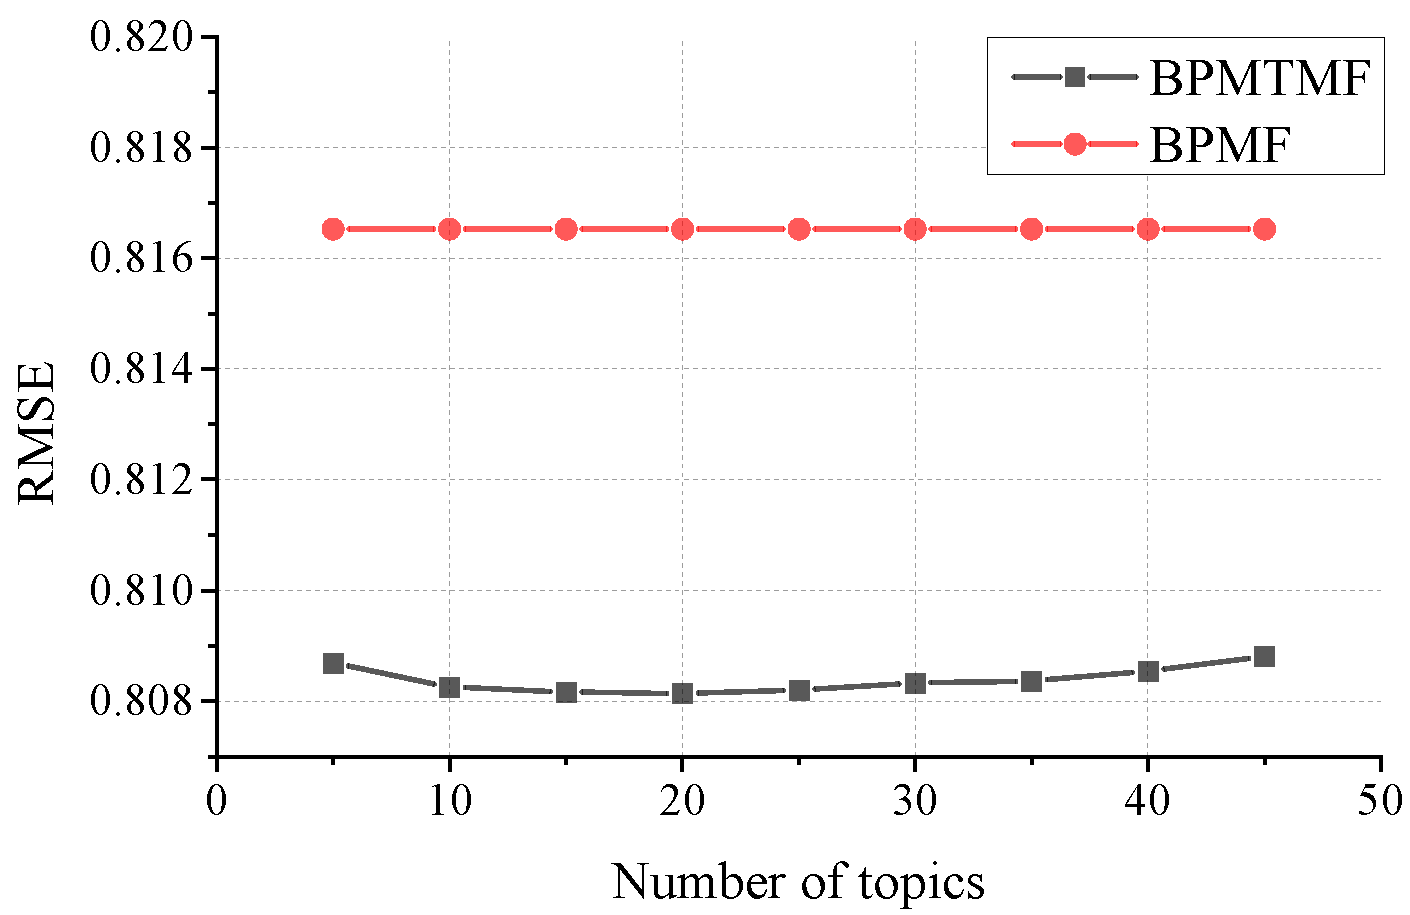
\includegraphics[width=0.75\textwidth]{Fig/bpmtmf/number}
	\caption{不同主题个数对推荐准确率的影响}
	\label{fig-bpmtmf-number}
\end{figure}
由于本章工作需要根据每个主题设置主题特定的用户隐藏特征向量和商品隐藏特征向量,因此本章提出的BPMTMF一个重要的参数是主题个数(也就是 $H$)。本小节实验以5为间隔在区间$[5,45]$上设置不同的主题个数$H$。图~\ref{fig-bpmtmf-number}展示了BPMTMF的RMSE性能。图中能观察到在主题个数符合$15\le H\le 25$时,BPMTMF取得的推荐准确率最高。作为对照,实验也测试了BPMF的性能,BPMF其实是只有一个主题的BPMTMF,是BPMTMF的一种特殊情形。可以看出,当主题个数$H=5$时,BPMTMF的推荐准确率已经远好于主题个数为1时的准确率。通过结合表~\ref{tab-bpmtmf-cluster}聚类分析能够看出利用多主题的矩阵分解模型能够有效地对用户和商品复杂的特性进行建模,从而提高预测评分的准确性。

\begin{figure}
	\centering
	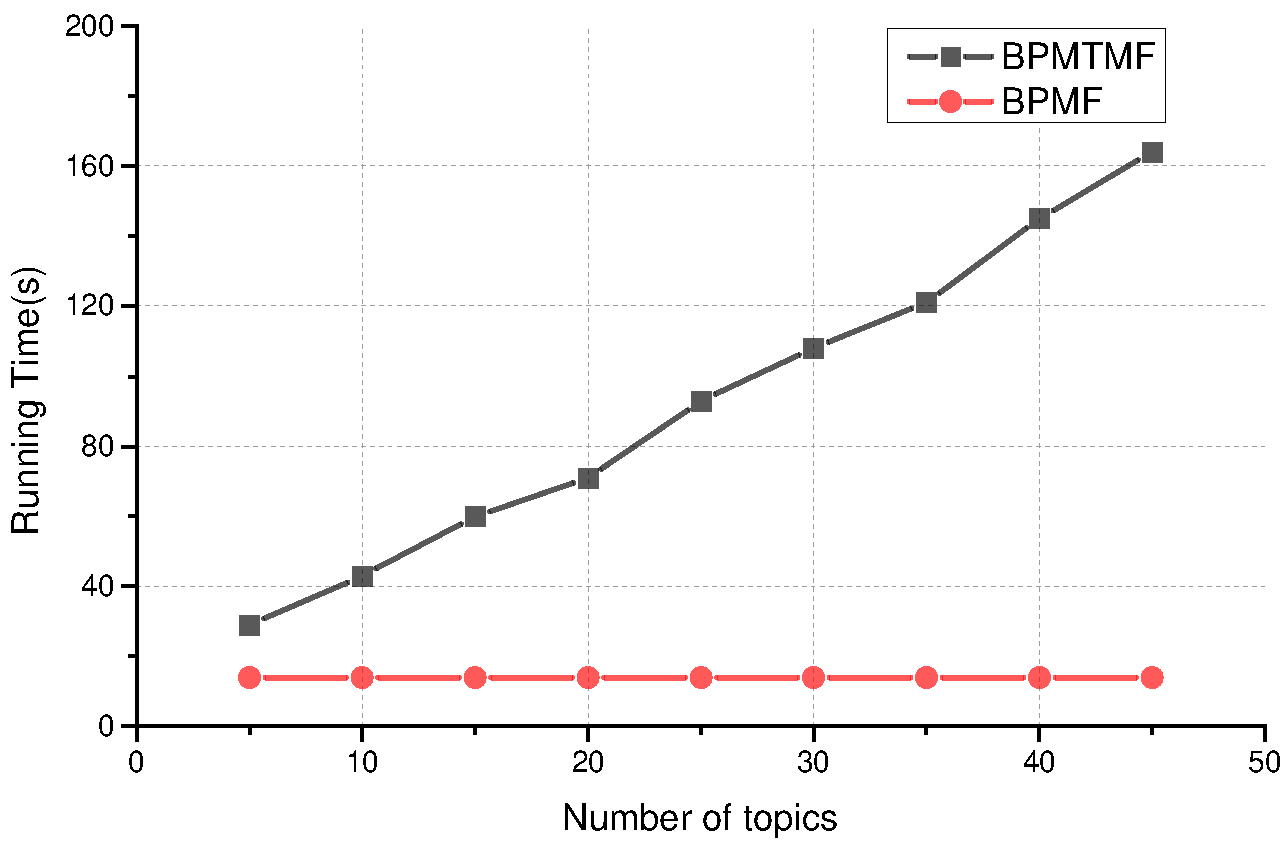
\includegraphics[width=0.75\textwidth]{Fig/bpmtmf/ktime}
	\caption{不同主题个数对模型训练时间的影响}
	\label{fig-bpmtmf-time}
\end{figure}

本小节实验同时也展示了BPMTMF每轮迭代的算法运行时间,如图~\ref{fig-bpmtmf-time}所示。该实验使用的电脑配置是Ubuntu系统,CPU为4-core Intel Xeon E5-1603 2.86GHz以及16G内存,使用Java编程语言实现BPMTMF。在之前的时间复杂度分析中,每一轮迭代本文模型BPMTMF的时间复杂度为$\mathcal{O}(KH|\mathbf{R}|+K^2|\mathbf{R}|+K^3HN+K^3HM)$。在数据集大小和隐藏特征向量维度不变的情况下,BPMTMF的时间复杂度与主题个数$H$成正比。从图~\ref{fig-bpmtmf-time}可以看出,实验结果也符合本章的时间复杂度理论分析。为了提高算法运行效率在以后工作中引入并行优化算法去加速参数学习过程。

\section{本章小结}
\label{sec-bpmtmf-conclusion}
本章提出了局部矩阵分解的概率形式,巧妙地融合概率矩阵分解和主题模型到同一个模型当中,进而提出全贝叶斯版本的概率多主题矩阵分解BPMTMF。本章同时也说明了之前一些非概率版本的局部矩阵分解模型和本章模型的紧密联系。本章工作在评分预测上能够更加有效地反映用户和商品复杂的内在特性,以及有更好的模型解释性。另外,在大规模真实数据集上的实验也表明了本章模型的有效性。

\clearpage
\phantom{s}
\clearpage